The user then clicks on the E21\_Person1 in the R2RML mapping and selects Augment Data to discover new data to integrate into artist records.  Karma then parses R2RML mappings in its repository that describe crm:E21\_Person for object and data properties.
Karma could look in a triple store for all the properties with subjects or objects of type crm:E21\_Person or even use OWL to reason about the properties of crm:E21\_Person.
That would be exhaustive and expensive and only serve to overwhelm the user with possibilities.
Instead, the R2RML mappings allow Karma to identify meaningful properties and present them to the user as illustrated in Figure~\ref{fig:search-screenshot}.

To aid the user, Karma also estimates how many of the user's artists have these properties in the triple store.  
Karma does this by testing the artists' URIs against Bloom filters that it created when generating RDF triples and then associated with the Predicate Object Maps of an R2RML mapping.  
Karma's estimation helps the user avoid an expensive and unfruitful join very cheaply since the Bloom filters trade a small false positive rate for a much smaller set data structure than a perfect hash, all while supporting arbitrary set operations.  
\begin{figure*}
\begin{center}
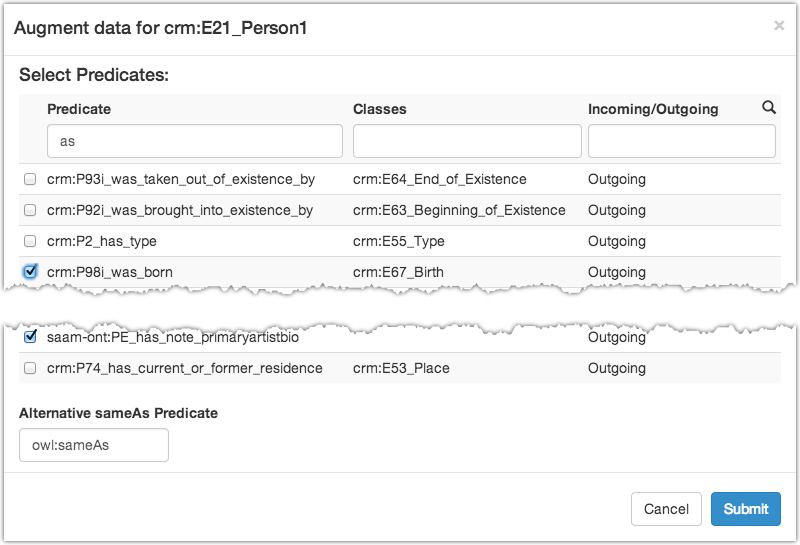
\includegraphics[width=4.9in]{images/5-search.png}
\vspace{-3mm}
\caption{A Karma user selects CIDOC CRM object and data properties discovered from other sources to augment crm:E21\_Person}
\vspace{-2mm}
\label{fig:search-screenshot}
\end{center}
\vspace{-1.5em}
\end{figure*}